\documentclass{beamer}

\usepackage[french]{babel}
\usepackage[T1]{fontenc}
\usepackage[utf8]{inputenc}

\usetheme{Warsaw}
\useoutertheme{infolines}

\usepackage{amsmath}
\usepackage{amssymb}
\usepackage{amsthm}
\usepackage{stmaryrd}

\usepackage[all]{xy}

%Les sous listes on des triangles
\setbeamertemplate{itemize item}[circle]
\setbeamertemplate{itemize subitem}[triangle]
%Les elements caché sont grisé
\beamertemplatetransparentcovered

\begin{document}

\title{Android - Les fondamentaux}
\author{Jérémy S. Cochoy}
\institute{INRIA Paris-Saclay | jeremy.cochoy@u-psud.fr}
\date{Octobre 2015}


\begin{frame}
\titlepage
\end{frame}

\begin{frame}
\tableofcontents
\end{frame}

\begin{frame}
\frametitle{La documentation}

\begin{block}{Votre nouveau livre de chevet.}
\begin{center}
\emph{https://developer.android.com/guide/index.html}
\end{center}
\end{block}

\end{frame}

\section{Applications}

\begin{frame}
\frametitle{Qu'est-ce qu'une application?}

\begin{itemize}
	\item Les applications android sont écrite en Java
	\item Le SDK créer un fichier APK (Android Package)
\end{itemize}

\end{frame}


\begin{frame}
\frametitle{Sandbox}

\begin{itemize}
	\item Un système multi-utilisateur, un user par app.
	\item Les fichiers de l'app ne sont accessible que par cet user.
	\item Chaque processus a sa propre VM.
\end{itemize}

Pour accéder à d'autres fichiers, une app requière des privilèges.

\end{frame}

\begin{frame}
\frametitle{Les composants}

\begin{center}
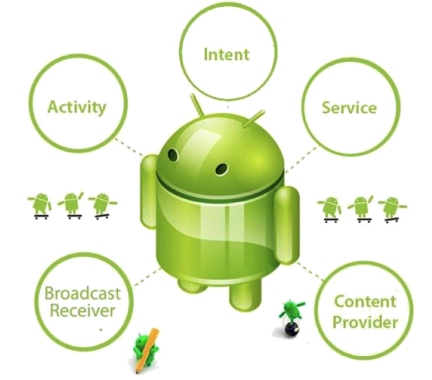
\includegraphics[scale=0.5]{components.png}
\end{center}
\end{frame}

\begin{frame}
\frametitle{Les composants}

\begin{block}{}
 Les composants sont les blocks élémentaires. Certains sont les entrypoint de l'application. Il y à 4 type de composants :
\end{block}

\begin{itemize}
	\item Activities
	\item Services
	\item Content providers
	\item Broadcast receivers
\end{itemize}

\end{frame}

\begin{frame}
\frametitle{Activities}

\begin{center}
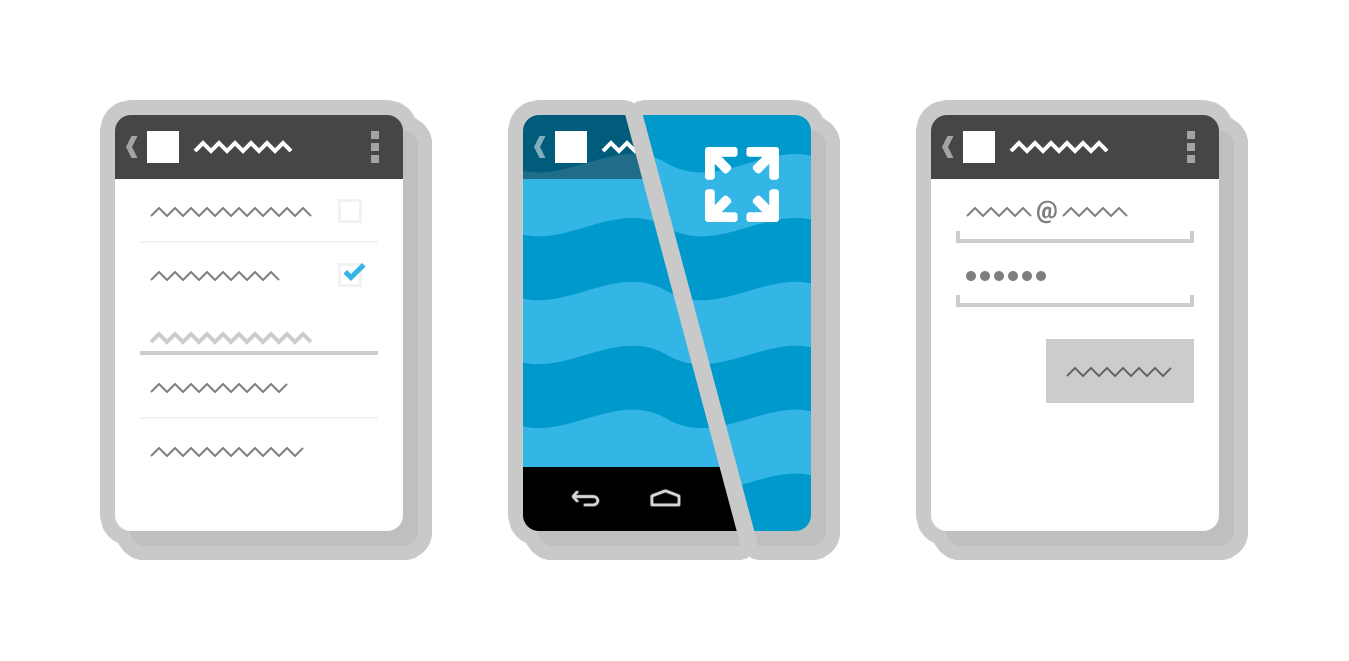
\includegraphics[scale=0.1]{c-activity.png}
\end{center}

\begin{block}{}
Une activité est un écran avec une interface utilisateur.

Ex : liste des mails, affichage d'un e-mail, etc.
\end{block}
\begin{block}{}
Une app peux lancer l'activité d'une autre app.

Ex : appareil photo.
\end{block}

\begin{block}{}
Une activité est implémenté comme une sous classe d'\verb!Activity!.
\end{block}
\end{frame}

\begin{frame}
\frametitle{Services}

\begin{center}
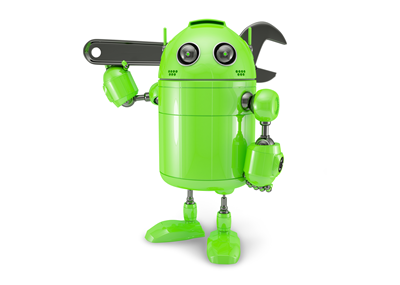
\includegraphics[scale=0.8]{c-services.png}
\end{center}


\begin{block}{}
Un service est un composant qui s’exécute en arrière plan.

Ex : musique, facebook messenger, etc.
\end{block}

\begin{block}{}
Un service est une instance d'une sous classe de \verb!Service!.
\end{block}
\end{frame}

\begin{frame}
\frametitle{Content providers}


\begin{center}
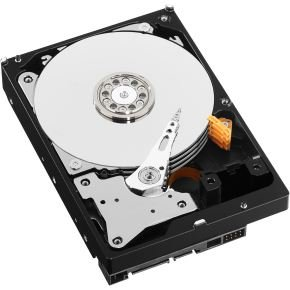
\includegraphics[scale=0.3]{c-content.jpg}
\end{center}


\begin{block}{}
Gère un ensemble de données partagé entre des applications. FS, SQLite, Cloud...

Ex : Les contactes de l'utilisateur.
\end{block}

\begin{block}{}
Un fournisseur de contenu  est implémenté comme une sous classe de \verb!ContentProvider!. Cette classe doit implémenter une API.
\end{block}
\end{frame}

\begin{frame}
\frametitle{Broadcast receiver}
\begin{block}{}
Un Broadcast receiver est un composant qui répond aux messages émis par le système, à l'intention de toute les applications. Une application peux aussi émettre un message.

Ex : Batterie faible, écran en veille, photo prise...
\end{block}

\begin{block}{}
En général, un broadcast receiver est un composant léger dont le seul but est de lancer une autre tache qui s'occupera du traitement (service, ou activité).
\end{block}

\begin{block}{}
Un broadcast receiver est implémenté comme sous classe de \verb!BroadcastReceiver!. Chaque message est délivrer sous la forme d'un objet \verb!Intent!.
\end{block}
\end{frame}

\begin{frame}
\frametitle{Appeler un composant}
\begin{center}
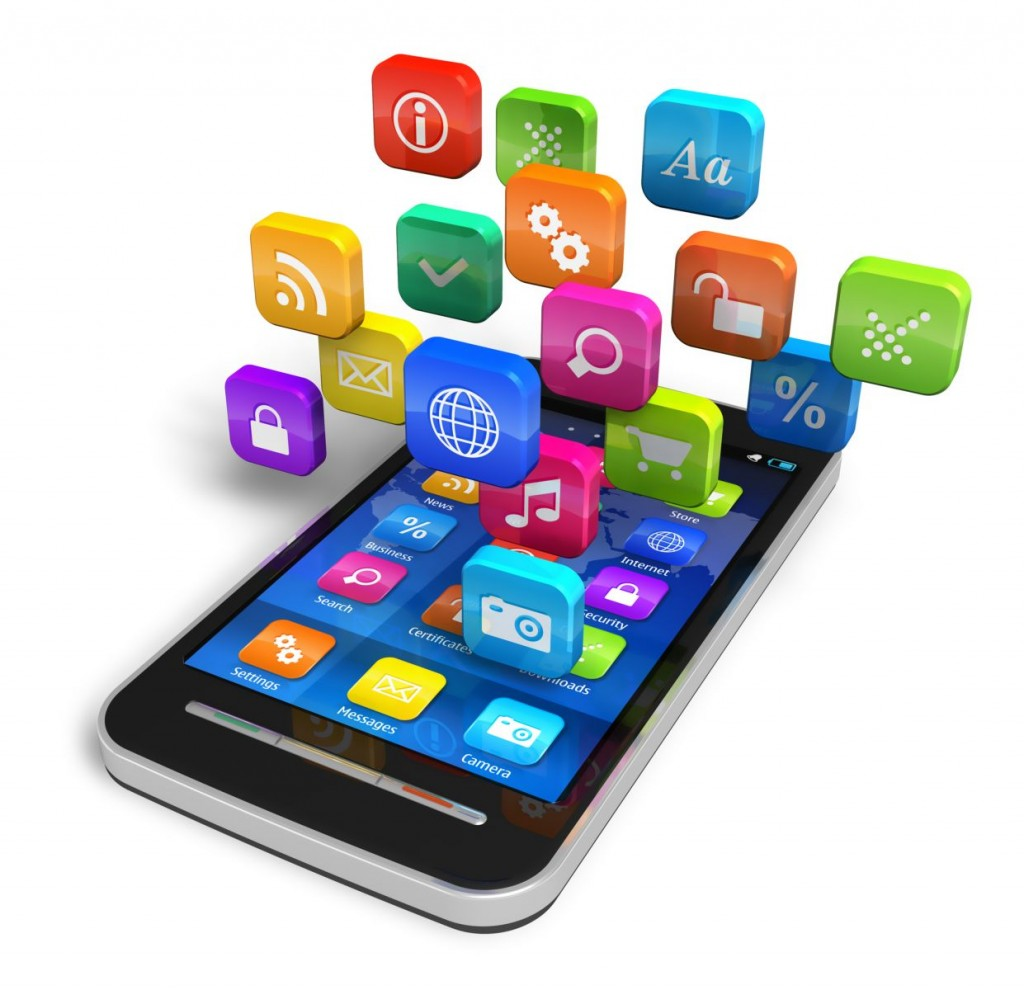
\includegraphics[scale=0.1]{app.jpg}
\end{center}

\begin{itemize}
\item Une app peux appeler le composant d'une autre app.
\item Chaque composant s'exécute dans l'app à laquelle il appartiens.
\item Il n'existe donc pas de \verb!main()! comme dans d'autres applications.
\end{itemize}

\end{frame}

\section{Le manifest}

\begin{frame}
\frametitle{A quoi sert le fichier manifest?}

\begin{itemize}
\item Liste les permissions requise pour exécuter l'application (liste de contactes, internet, appareille photo, ...)
\item Déclare l'API minimal sous la quel l'application peux s'exécuter
\item Déclare les fonctionnalités matériel requise/utilisé par l'application (bluetouth, multitouch, ...)
\item Bibliothèques utilisés (ex : Google Maps library)
\item Liste les composants de l'application
\item et encore d'autres choses...
\end{itemize}

\end{frame}


\section{Les activités}

\section{Les intentions}

\begin{frame}
\begin{center}
Pour me contacter : jeremy.cochoy@u-psud.fr, merci et à bientôt.


\includegraphics[scale=0.18]{android.jpg}
\end{center}
\end{frame}

\end{document}
